%%%%%%%%%%%%%%%%%%%%%%%%%%%%%%%%%%%%%%%%%%%%%%%%%%%%%%%%%%%%%%%%%%%%%%
%%  Copyright by Wenliang Du.                                       %%
%%  This work is licensed under the Creative Commons                %%
%%  Attribution-NonCommercial-ShareAlike 4.0 International License. %%
%%  To view a copy of this license, visit                           %%
%%  http://creativecommons.org/licenses/by-nc-sa/4.0/.              %%
%%%%%%%%%%%%%%%%%%%%%%%%%%%%%%%%%%%%%%%%%%%%%%%%%%%%%%%%%%%%%%%%%%%%%%

\newcommand{\commonfolder}{../../common-files}

\documentclass[11pt]{article}

\usepackage[most]{tcolorbox}
\usepackage{times}
\usepackage{epsf}
\usepackage{epsfig}
\usepackage{amsmath, alltt, amssymb, xspace}
\usepackage{wrapfig}
\usepackage{fancyhdr}
\usepackage{url}
\usepackage{verbatim}
\usepackage{fancyvrb}
\usepackage{adjustbox}
\usepackage{listings}
\usepackage{color}
\usepackage{subfigure}
\usepackage{cite}
\usepackage{sidecap}
\usepackage{pifont}
\usepackage{mdframed}
\usepackage{textcomp}
\usepackage{enumitem}
\usepackage{hyperref}


% Horizontal alignment
\topmargin      -0.50in  % distance to headers
\oddsidemargin  0.0in
\evensidemargin 0.0in
\textwidth      6.5in
\textheight     8.9in 

\newcommand{\todo}[1]{
\vspace{0.1in}
\fbox{\parbox{6in}{TODO: #1}}
\vspace{0.1in}
}


\newcommand{\unix}{{\tt Unix}\xspace}
\newcommand{\linux}{{\tt Linux}\xspace}
\newcommand{\minix}{{\tt Minix}\xspace}
\newcommand{\ubuntu}{{\tt Ubuntu}\xspace}
\newcommand{\setuid}{{\tt Set-UID}\xspace}
\newcommand{\openssl} {\texttt{openssl}}


\pagestyle{fancy}
\lhead{\bfseries SEED Labs}
\chead{}
\rhead{\small \thepage}
\lfoot{}
\cfoot{}
\rfoot{}


\definecolor{dkgreen}{rgb}{0,0.6,0}
\definecolor{gray}{rgb}{0.5,0.5,0.5}
\definecolor{mauve}{rgb}{0.58,0,0.82}
\definecolor{lightgray}{gray}{0.90}


\lstset{%
  frame=none,
  language=,
  backgroundcolor=\color{lightgray},
  aboveskip=3mm,
  belowskip=3mm,
  showstringspaces=false,
%  columns=flexible,
  basicstyle={\small\ttfamily},
  numbers=none,
  numberstyle=\tiny\color{gray},
  keywordstyle=\color{blue},
  commentstyle=\color{dkgreen},
  stringstyle=\color{mauve},
  breaklines=true,
  breakatwhitespace=true,
  tabsize=3,
  columns=fullflexible,
  keepspaces=true,
  escapeinside={(*@}{@*)}
}

\newcommand{\newnote}[1]{
\vspace{0.1in}
\noindent
\fbox{\parbox{1.0\textwidth}{\textbf{Note:} #1}}
%\vspace{0.1in}
}


%% Submission
\newcommand{\seedsubmission}{
Debe enviar un informe de laboratorio detallado, con capturas de pantalla, para describir lo que ha hecho y lo que ha observado.
También debe proporcionar una explicación a las observaciones que sean interesantes o sorprendentes.
Enumere también los fragmentos de código más importantes seguidos de una explicación. No recibirán créditos aquellos fragmentos de códigos que no sean explicados.}

%% Book
\newcommand{\seedbook}{\textit{Computer \& Internet Security: A Hands-on Approach}, 2nd
Edition, by Wenliang Du. Para más detalles \url{https://www.handsonsecurity.net}.\xspace}

%% Videos
\newcommand{\seedisvideo}{\textit{Internet Security: A Hands-on Approach},
by Wenliang Du. Para más detalles \url{https://www.handsonsecurity.net/video.html}.\xspace}

\newcommand{\seedcsvideo}{\textit{Computer Security: A Hands-on Approach},
by Wenliang Du. Para más detalles \url{https://www.handsonsecurity.net/video.html}.\xspace}

%% Lab Environment
\newcommand{\seedenvironment}{Este laboratorio ha sido testeado en nuestra imagen pre-compilada de una VM con Ubuntu 16.04, que puede ser descargada del sitio oficial de SEED.\xspace}

\newcommand{\seedenvironmentA}{Este laboratorio ha sido testeado en nuestra imagen pre-compilada de una VM con Ubuntu 16.04, que puede ser descargada del sitio oficial de SEED.\xspace}

\newcommand{\seedenvironmentB}{Este laboratorio ha sido testeado en nuestra imagen pre-compilada de una VM con Ubuntu 20.04, que puede ser descargada del sitio oficial de SEED .\xspace}

\newcommand{\seedenvironmentC}{Este laboratorio ha sido testeado en nuestra imagen pre-compilada de una VM con Ubuntu 20.04, que puede ser descargada del sitio oficial de SEED. Sin embargo, la mayoría de nuestros laboratorios pueden ser realizados en la nube para esto Ud. puede leer nuestra guía que explica como crear una VM de SEED en la nube.\xspace}

\newcommand{\seedenvironmentAB}{
Este laboratorio ha sido testeado en nuestras imagenes pre-compiladas de una VM con Ubuntu 16.04 y otra con Ubuntu 20.04, que pueden ser descargadas del sitio oficial de SEED.\xspace}

\newcommand{\nodependency}{Dado que utilizamos contenedores para configurar el entorno de laboratorio, este laboratorio no depende estrictamente de la VM de SEED. Puede hacer este laboratorio utilizando otras máquinas virtuales, máquinas físicas o máquinas virtuales en la nube.\xspace}

\newcommand{\adddns}{You do need to add the required IP address mapping to
the \texttt{/etc/hosts} file.\xspace}






\newcommand{\seedlabcopyright}[1]{
\vspace{0.1in}
\fbox{\parbox{6in}{\small Copyright \copyright\ {#1}\ \ by Wenliang Du.\\
      Este trabajo se encuentra bajo licencia Creative Commons.
       Attribution-NonCommercial-ShareAlike 4.0 International License.
       Si ud. remezcla, transforma y construye a partir de este material,
       Este aviso de derechos de autor debe dejarse intacto o reproducirse de una manera que sea razonable para el medio en el que se vuelve a publicar el trabajo.
       }}
\vspace{0.1in}
}







\newcommand{\dnsFigs}{./Figs}
\lhead{\bfseries SEED Labs -- DNS In a Box}


\def \code#1 {\fbox{\scriptsize{\texttt{#1}}}}

\newcommand{\bankcom}{\url{bank32.com}\xspace}
\newcommand{\wwwbank}{\url{www.bank32.com}\xspace}
\newcommand{\examplenet}{\url{example.net}\xspace}
\newcommand{\wwwexample}{\url{www.example.net}\xspace}
\newcommand{\dockerfile}{\texttt{Dockerfile}\xspace}
\newcommand{\bind}{\texttt{BIND9}\xspace}

\begin{document}

\begin{center}
{\LARGE SEED Lab: DNS In a Box}
\end{center}

\seedlabcopyright{2020}



% *******************************************
% SECTION
% ******************************************* 
\section{Descripción del Laboratorio}

DNS (Domain Name System o Sistema de nombre de Dominios) es la guía de teléfono de la Internet; se encarga de traducir los hostnames a direcciones IP (y visce versa). Esta traducción se hace a través de la resolución DNS, esta ocurre detrás de escena. El proceso de resolución involucra muchos nameservers, incluyendo los nameservers raíz, servidores TLD y los servidores de dominio finales. Estos nameservers pertenecientes al sistema global DNS, es una parte fundamental de la infraestructura de la Internet.

Par ayudar a que los estudiantes entiendan como estos nameservers funcionan de manera conjunta para así forma la infraestructura, crearemos un sistema DNS en miniatura llamado \textit{DNS in a Box}. Como sugiere su nombre, se correrá un sistema DNS que contará con múltiples nameservers dentro de una sóla máquina. Esto se logrará usando la tecnología de los contenedores.

Aunque este sistema es pequeño, contiene todos los elementos esencial de una infraestructura real DNS. Construyendo tal sistema, los estudiantes tendrán un conocimiento más en profundidad sobre como funciona el protocolo DNS.
Aunque este laboratorio no se trata de la seguridad, contiene la bases para otros laboratorios de SEED.

Este laboratorio cubre los siguientes tópicos:

\begin{itemize}[noitemsep]
\item DNS y su funcionamiento
\item El proceso de consulta DNS
\item Servidores raíz y TLDs
\item Contenedores Docker y Docker Compose
\end{itemize}



\paragraph{Lecturas y videos.}
Para una cobertura más detallada sobre el protocolo DNS puede consultar:

\begin{itemize}
\item Capítulo 18 del libro de SEED, \seedbook
\item Seccióon 7 del curso de SEED en Udemy, \seedisvideo
\end{itemize}


\paragraph{Entorno de Laboratorio.} 
\seedenvironmentB
\nodependency





% *******************************************
% SECTION
% *******************************************
\section{Setup del Laboratorio} 


\begin{figure}[htb]
\begin{center}
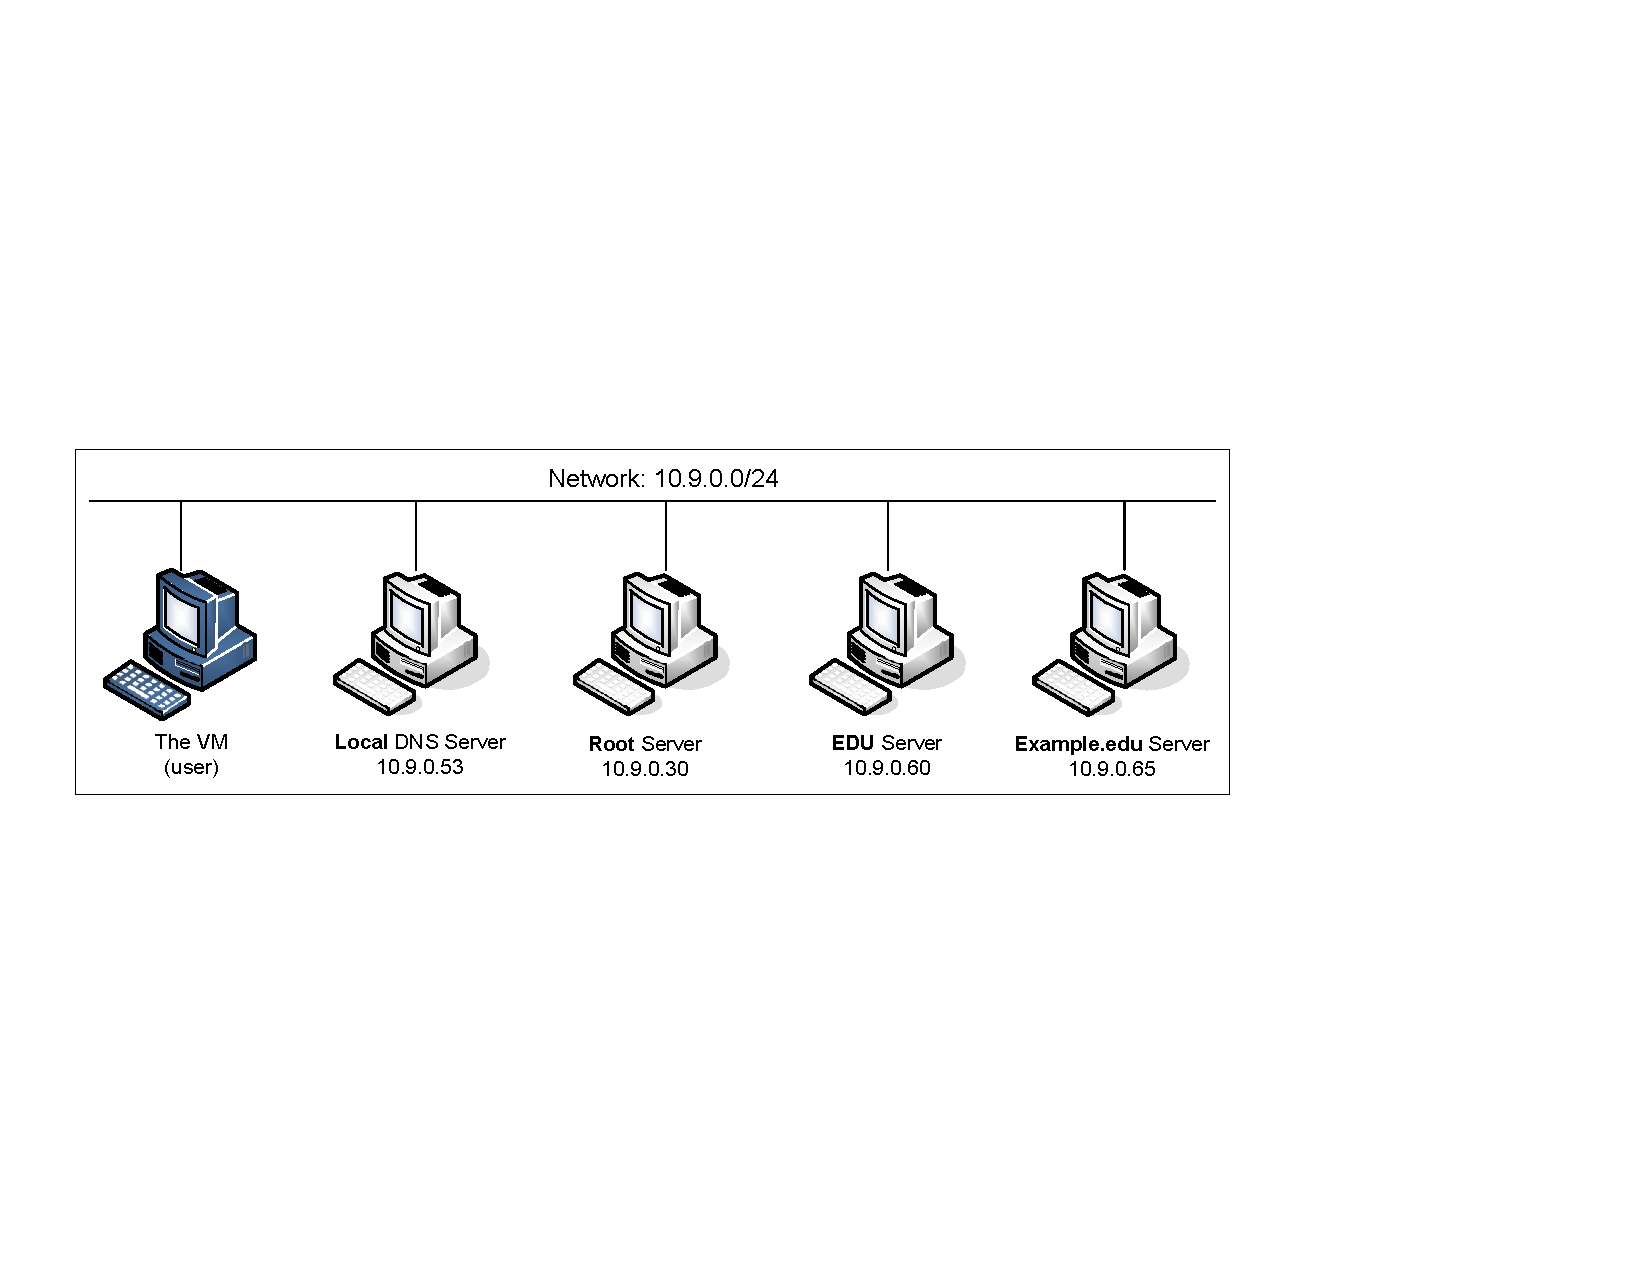
\includegraphics[width=0.95\textwidth]{Figs/DNS-in-a-box.pdf}
\end{center}
\caption{Una infraestructura de DNS simplificada}
\label{dns:fig:dns-in-a-box}
\end{figure}

En este laboratorio, construiremoss una infraestructura DNS simplificada. Empezaremos por una pequeña y gradualmente la iremos escalando.
El primer sistema DNS que haremos consistirá en cuatro nameservers, cada uno representará un rol específico en esta infraestructura DNS.
En el mundo real, estos nameservers se encuentran en redes diferentes, pero por un tema de simplicidad, en este laboratorio, los ubicaremos en la misma red.
La Figura \ref{dns:fig:dns-in-a-box} ilustra el setup del sistema.
Usaremos contenedores para correr estos nameservers.

% -------------------------------------------
% SUBSECTION
% -------------------------------------------
\subsection{Setup del Contenedor y sus Comandos}

%%%%%%%%%%%%%%%%%%%%%%%%%%%%%%%%%%%%%%%%%%%%
Para empezar a preparar el contenedor, deberá descargarse el archivo \texttt{Labsetup.zip} ubicado en el laboratorio correspondiente dentro del sitio web oficial y copiarlo dentro de la Máquina Virtual prevista por SEED. Una vez descargado deberá descomprimirlo y entrar dentro del directorio \texttt{Labsetup} donde encontrará el archivo \texttt{docker-compose.yml} que servirá para setear el entorno de laboratorio. Para una información más detallada sobre el archivo \texttt{Dockerfile} y otros archivos relacionados, puede encontrarla dentro del Manual de Usuario del laboratorio en uso, en el sitio web oficial de SEED.

Si esta es su primera experiencia haciendo el setup del laboratorio usando contenedores es recomendable que lea el manual anteriormente mencionado.

A continuación, se muestran los comandos más usados en Docker y Compose.
Debido a que estos comandos serán usados con mucha frecuencia, hemos creados un conjunto de alias para los mismos, ubicados en del archivo \texttt{.bashrc} dentro de la Máquina Virtual provista por SEED (Ubuntu 20.04)

\begin{lstlisting}
$ docker-compose build  # Build the container image
$ docker-compose up     # Start the container
$ docker-compose down   # Shut down the container

// Aliases for the Compose commands above
$ dcbuild       # Alias for: docker-compose build
$ dcup          # Alias for: docker-compose up
$ dcdown        # Alias for: docker-compose down
\end{lstlisting}


Dado que todos los contenedores estarán corriendo en un segundo plano. Necesitamos correr comandos para interactuar con los mismos, una de las operaciones fundamentales es obtener una shell en el contenedor. 
Para este propósito usaremos \texttt{"docker ps"} para encontrar el ID del contenedor deseado y ingresaremos \texttt{"docker exec"} para correr una shell en ese contenedor.
Hemos creado un alias para ello dentro del archivo \texttt{.bashrc}

\begin{lstlisting}
$ dockps        // Alias for: docker ps --format "{{.ID}}  {{.Names}}" 
$ docksh <id>   // Alias for: docker exec -it <id> /bin/bash

// The following example shows how to get a shell inside hostC
$ dockps
b1004832e275  hostA-10.9.0.5
0af4ea7a3e2e  hostB-10.9.0.6
9652715c8e0a  hostC-10.9.0.7

$ docksh 96
root@9652715c8e0a:/#  

// Note: If a docker command requires a container ID, you do not need to 
//       type the entire ID string. Typing the first few characters will 
//       be sufficient, as long as they are unique among all the containers. 
\end{lstlisting}

En caso de problemas configurando el entorno, por favor consulte la sección ``Common Problems'' en el manual ofrecido por SEED. 


%%%%%%%%%%%%%%%%%%%%%%%%%%%%%%%%%%%%%%%%%%%%



% -------------------------------------------
% SUBSECTION
% -------------------------------------------
\subsection{El archivo Docker Compose} 

Our DNS system includes the four nameservers. 
The purpose of these four nameservers are summarized in the following:

\begin{itemize}[nosep]
\item Local DNS server: conduct the DNS resolution process for other computers.
\item Root server: a nameserver serving the root zone.
\item \texttt{edu} server: nameserver serving the \texttt{edu} zone, a Top Level Domain (TLD).  
\item \texttt{example.edu} server: nameserver serving the \texttt{example.edu} zone. 
\end{itemize}


We use a container for each of the nameservers above. 
How these containers are built and run is described in 
the \texttt{docker-compose.yml} file, which is included in
the lab setup file. Inside this file, we create a network \texttt{10.9.0.0/24}
and four containers: each entry in the \texttt{services} section represents
a container. We also assign IP addresses to those containers. 
See the following snippet:

\begin{lstlisting}
services:
  seed_base_router:                       (*@\ding{80}@*)
    build: ./base_image
    image: seed-base-image-bind
    container_name: seed-base-bind
    command: " echo 'exiting ...' "

  example_edu_server:
    build:
        context: ./nameserver
        args:
            BIND_CONF_DIR: edu.example
    image: example-edu-server
    container_name: example-edu-10.9.0.65
    tty: true
    networks:
      seed-net:
        ipv4_address: 10.9.0.65

  edu_server:        ... (omitted, similar to example_edu_server) ...
        ipv4_address: 10.9.0.60
  root_server:       ... (omitted, similar to example_edu_server) ...
        ipv4_address: 10.9.0.30
  local_dns_server:  ... (omitted, similar to example_edu_server) ...
        ipv4_address: 10.9.0.53
\end{lstlisting}

Line \ding{80} specifies a base image, which basically builds an 
image based on the \path{handsonsecurity/seed-server:bind} image 
we placed on Docker Hub (see \texttt{Dockerfile} in the \texttt{base\_image} folder). 
Although all the nameservers can directly build their containers using
this base image from the Docker Hub, to reduce
the number of access to the Docker Hub (the company
puts a limit on how many accesses one can make
during a six-hour time window), we first build a
local base image using the one from Docker Hub, and then
use the local base image to build the rest of the
container images in this lab.


% -------------------------------------------
% SUBSECTION
% -------------------------------------------
\subsection{Las Imagenes Docker} 

Except for the local DNS server, all the nameservers use the same 
folder (\texttt{nameserver}) to build Docker images. The 
\texttt{Dockerfile} is shown in the following:  

\begin{lstlisting}
FROM seed-base-image-bind                         (*@\ding{202}@*)

ARG BIND_CONF_DIR

# Copy the BIND confirguration files
COPY named.conf named.conf.options  /etc/bind/    (*@\ding{203}@*)
COPY ${BIND_CONF_DIR}     /etc/bind/              (*@\ding{204}@*)

# Start the nameserver
CMD service named start  && tail -f /dev/null
\end{lstlisting}

Line \ding{202} indicates this is local image (the base image).
Line \ding{203} copies the BIND 9's configuration files to
the \texttt{/etc/bind} folder inside the container. These two files
are the same for all the nameservers, but each nameserver's 
does have its own zone files. That is why we use 
the \texttt{BIND\_CONF\_DIR} argument (Line \ding{204}) to 
indicate which configuration folder should be used (there is 
a folder for each nameserver). The value of \texttt{BIND\_CONF\_DIR} 
is set in the Compose file. 


\paragraph{Local DNS server.}
The container image for the local DNS server is quite similar to
that in the nameservers. We will explain the difference later, 
as building the image is one of the tasks. 




% *******************************************
% SECTION
% *******************************************
\section{Task l: Building the nameserver for \texttt{example.edu}}

In this task, we will build a nameserver for a domain 
called \texttt{example.edu}. The container files are 
put inside the \texttt{nameserver} folder. 
The configuration files for this particular domain
is placed inside the \path{edu.example} sub-folder.  


\paragraph{Step 1. Adding the zone entry}. To host
a server for the \texttt{example.edu} domain, we need to
add a zone entry to the BIND 9's configuration file \texttt{named.conf}, 
so it knows what zones it is going to host. For convenience,
we will add the entry to the \path{named.conf.seedlabs} file, which
is included in our modified \texttt{named.conf} file.


This entry indicates that the current nameserver 
is the master server for this domain, and the zone file is 
specified in the \texttt{file} entry.  


\begin{lstlisting}
zone "example.edu" {
        type master;
        file "/etc/bind/example.edu.db";
};
\end{lstlisting}


\paragraph{Step 2. Creating the zone file}. 
When building the docker image, the zone file 
\path{example.edu.db} will be copied into
the \path{/etc/bind} folder of the container. 
To get students started, we have provided some 
information in this zone file, but students need to make 
all then necessary changes.

\begin{lstlisting}
$TTL 3D
@       IN      SOA   ns.example.edu. admin.example.edu. (
                2008111001
                8H
                2H
                4W
                1D)

; Records for this nameserver (you need to make changes)
@               IN   NS    ns.example.edu.
ns.example.edu  IN   A     1.2.3.4


; IP addresses for the hostnames in the example.du domain
@       IN      A     1.2.3.5
www     IN      A     1.2.3.5
xyz     IN      A     1.2.3.6
*       IN      A     1.2.3.7
\end{lstlisting}
 


\paragraph{Step 3. Testing.} Using \texttt{docker-compose} commands
to build and start all the containers. 
Once the containers are running,
run the following command from your VM (i.e., outside of the 
container). We use the \texttt{@10.9.0.65} option to send our DNS query
directly to texttt{10.9.0.65}, which is the IP
address of the \texttt{example.edu} nameserver in our setup. 
If everything is done correctly, you can get the IP address specified
in your zone file. Please report your observations.

\begin{lstlisting}
$ dig @10.9.0.65 www.example.edu
... 
;; ANSWER SECTION:
www.example.edu.    259200   IN  A   (*@\textbf{1.2.3.5}@*)
...
\end{lstlisting}





% *******************************************
% SECTION
% *******************************************
\section{Task 2: Building the \texttt{edu} TLD server}


In this task, we will build a nameserver for a TLD domain, 
the \texttt{edu} domain.
We will modify the files in the \texttt{nameserver/edu} folder. 
First, we need to  add the following zone entry to the
\path{named.conf.seedlabs} file. This entry indicates that the current nameserver
is the master server for this domain, and the zone file is
specified in the \texttt{file} entry.

\begin{lstlisting}
zone "edu" {
        type master;
        file "/etc/bind/edu.db";
};
\end{lstlisting}


\paragraph{Creating the zone file.} Next, we need to
add records to the zone file. 
We have already created the zone file \texttt{edu.db},
but it is incomplete. Students should make all the 
necessary changes. 

All the nameservers within the \texttt{edu} domain
must register their nameservers with this 
TLD server; otherwise, nobody can find them. As an example,
we have added two records for the \texttt{syr.edu} domain: 
an \texttt{NS} record and an \texttt{A} record.
The \texttt{NS} record specifies the nameserver for the 
\texttt{syr.edu} domain, while the \texttt{A} record
specifies the IP address of the nameserver. The
data used in the records are real data, as it simulates
the fact the \texttt{syr.edu} domain has registered 
itself with our \texttt{edu} TLD server.

\begin{lstlisting}
; Real records for syr.edu
syr.edu.                IN      NS      ns1.syr.edu.
ns1.syr.edu.            IN      A       128.230.12.8
\end{lstlisting}
 

\paragraph{Lab Task.}
Students need to do the following tasks: (1) register 
your \texttt{example.edu} nameserver with this TLD server;
(2) choose three real domain names, and register them
with this TLD server. You can find the nameserver of a domain
using \texttt{"dig <name> NS"} (e.g., \texttt{"dig syr.edu NS"}). 


Using \texttt{docker-compose} commands, students can 
build and start all the containers. 
Once the containers are running,
run the following \texttt{dig} commands from your VM to
send DNS queries to the \texttt{edu} nameserver (its IP address
is \texttt{10.9.0.60} in our setup). 
Please report your observations. 


\begin{lstlisting}
$ dig @10.9.0.60 www.example.edu
$ dig @10.9.0.60 www.syr.edu
$ dig @10.9.0.60 <the other three domains you have chosen>
$ dig @10.9.0.60 <a domain not included in your zone file>
\end{lstlisting}

It should be noted, the \texttt{edu} TLD server is configured 
not to conduct the recursive query, so it will only tell you
the nameserver for the domain name in the query; it will not
resolve the query for you. In the last command, you should
try some domains (ended with \texttt{edu}) that are not included in your zone file. 


% *******************************************
% SECTION
% *******************************************
\section{Task 4: Building root server}


In this task, we will build a nameserver for the 
root zone. All TLD nameservers need to register
with the root nameserver, so they can be found
in the DNS query process. 
In our container, the root zone is defined in 
\texttt{bind.conf.seedlabs}, which loads the records 
from the zone file \texttt{root.db}. 


For every TLD zone that we would like to include in our 
miniature DNS system, we need to add at least two records
in the zone file, including an \texttt{NS} record 
and an \texttt{A} record.  In the following example,
we have added the nameserver information for the 
\texttt{com} and \texttt{net} zones (the data in the records are real data).
These two zones are managed by the same company, so they share the 
same set of nameservers (we have only included one nameserver).

\begin{lstlisting}
com.                 IN   NS   a.gtld-servers.net.
net.                 IN   NS   a.gtld-servers.net.
a.gtld-servers.net.  IN   A    192.5.6.30
\end{lstlisting}
 

\paragraph{Lab task.} Students need to add records to the 
zone file \texttt{root.db} to satisfy the following requirements:  

\begin{itemize}[nosep]
\item Register your \texttt{edu} nameserver with this root server.

\item Choose two more real TLD names, and register them
with this TLD server. One of the TLDs should be 
a country-code TLD (ccTLD), which is the root for 
a country. You can find the nameserver of a TLD domain
using \texttt{"dig <tld> NS"} (e.g., \texttt{"dig com NS"}).
You can also find all the TLD information from
\url{https://www.internic.net/domain/root.zone}.
\end{itemize}
 

Using \texttt{docker-compose} commands, students can
build and start all the containers. 
Once the containers are running,
run the \texttt{dig} command from your VM to
send DNS queries to the root nameserver (using 
\texttt{"dig @10.9.0.30"}). Please use the 
testing to demonstrate that your DNS setup 
is working as expected. 


% *******************************************
% SECTION
% *******************************************
\section{Task 5: Building the Local DNS Server} 

When a computer needs to resolve the IP address from a hostname (or vice versa),
it sends a request to its helper, which is called local DNS server (it
does not need to be local).  This local DNS server will conduct the 
entire DNS resolution process, and then send the result back to the computer. 
In this task, we will set up this local DNS server. 


\paragraph{The root hint file.}
If the local DNS server cannot find the answer from its cache, it 
will go through an iterative process to get the answer from outside 
nameservers.  The process starts from the root server. 
Therefore, the local DNS server needs to
know the IP address of the root servers. 


In \path{/etc/bind/named.conf.default-zones}, which is included 
in \bind's configuration file \path{/etc/bind/named.conf}, there is an 
entry for the root zone. This entry specifies a hint file for the
root zone, and that is how the local DNS server knows the IP address of the
root server. 


\begin{lstlisting}
zone "." {
	type hint;
	file "/usr/share/dns/root.hints";
};
\end{lstlisting}
 
The root hint file specifies the nameservers for the 
root zone (there are 13 nameservers for the root zone). The 
IP address (v4 and v6) for these nameservers are provided in this file. 
The following example shows a snippet of the file. 


\begin{lstlisting}
.                        3600000      NS    A.ROOT-SERVERS.NET.
A.ROOT-SERVERS.NET.      3600000      A     198.41.0.4
A.ROOT-SERVERS.NET.      3600000      AAAA  2001:503:ba3e::2:30
...
\end{lstlisting}

Inside our \texttt{local\_dns\_server} folder in the lab setup file,
we have created an empty file called \texttt{root.hints}. This file 
will be copied into the \path{/usr/share/dns/} folder when
we build the container image for the Local DNS server. 
You need to add records to this file, so your local DNS server 
can use your root server, instead of using the ones in the real world.



\paragraph{Testing.} Using \texttt{docker-compose} commands
to build and start all the containers.
Once the containers are running,
run the following \texttt{"dig @10.9.0.53"} commands from your VM to
send DNS queries to the local DNS nameserver (its IP address
is \texttt{10.9.0.53} in our setup). 
Please report your observations.

\begin{lstlisting}
$ dig @10.9.0.53 www.example.edu
$ dig @10.9.0.53 www.example.com
$ dig @10.9.0.53 www.example.net
$ dig @10.9.0.53 www.syr.edu
$ dig @10.9.0.53 www.xyz.<TLD registered with your root server>
$ dig @10.9.0.53 www.xyz.<TLD not registered with your root server>
\end{lstlisting}



% *******************************************
% SECTION
% *******************************************
\section{Task 6: Configure our VM to use this local DNS server} 

So far, we need to use \texttt{@<ip>} in our \texttt{dig} command
to indicate what DNS server the \texttt{dig} command should talk to. While this 
is not an issue for \texttt{dig}, it is a problem for other software that 
depends on DNS. We need to tell the operating system that the 
DNS server container built in this task is the system's 
local DNS server. 

This is achieved by changing
the resolver configuration file~(\texttt{/etc/resolv.conf}) of the user machine,
so the container's IP address is added as the first \texttt{nameserver} entry in the file, i.e.,
this server will be used as the primary DNS server.
Unfortunately, our provided VM uses the Dynamic Host Configuration Protocol (DHCP) to obtain
network configuration parameters, such as IP address, local DNS server, etc.
DHCP clients will overwrite \texttt{/etc/resolv.conf} with the information
provided by the DHCP server.

One way to get our information into \texttt{/etc/resolv.conf} without worrying about
the DHCP is to add the following entry to the \path{/etc/resolvconf/resolv.conf.d/head}
file:

\begin{lstlisting}
Add the following entry to /etc/resolvconf/resolv.conf.d/head
  nameserver 10.9.0.53

Run the following command for the change to take effect
$ sudo resolvconf -u
\end{lstlisting}

The content of the head file will be prepended to the dynamically generated resolver
configuration file. Normally, this is just a comment line (the comment in
\texttt{/etc/resolv.conf} comes from this head file).


After you finish configuring the user machine, repeat 
the testing commands in Task 5, but this time, do not 
include the \texttt{@<ip>} in the command. Pay attention to 
the highlighted IP address to check whether the response does 
come from your container. If the setup is unsuccessful,
the IP will be different.

\begin{lstlisting}
$ dig abc.example.edu

...
;; ANSWER SECTION:
abc.example.edu.	259200	IN	A	1.2.3.7

;; Query time: 3 msec
;; SERVER: (*@\textbf{10.9.0.53}@*)#53(10.9.0.53)
...
\end{lstlisting}
 

\paragraph{\ding{72}\ding{72} Note (very very important) \ding{72}\ding{72}.} 
After finishing the lab, please do remember to remove the added entry
from \path{/etc/resolvconf/resolv.conf.d/head}; otherwise, it will 
cause lot of problems for your future labs. If in the future,
you have trouble connecting to the Internet, but your network is fine, 
the chances are that you may have forgotten to remove this entry, and it 
messes up the DNS query process. This happens to me many times,
as I often forgot to remove the entry.


% *******************************************
% SECTION
% ******************************************* 
\section{Task 7: Making It More Realistic}


In this task, we will make our miniature DNS system
a little bit more realistic by adding the following 
nameservers or records to our system. 


\begin{itemize}
\item Adding 2 more root servers. The real-world DNS system has 13 different 
IP address for the root server. We will create 3 in this lab.


\item Pick two of the TLDs registered with your root server, 
build a second-level domain for each of them, use your last name as the domain name. 
For example, if your last name is \texttt{Smith}, you need to build the 
nameservers for the \texttt{smith.<tld1>} and \texttt{smith.<tld2>} domains,
You need to host both domains on the same nameserver. 
\end{itemize}




%Note: try to avoid using \texttt{com} and \texttt{net}. It 
%is harder, because they depend on each other.

 


% *******************************************
% SECTION
% ******************************************* 
\section{Informe del Laboratorio}

%%%%%%%%%%%%%%%%%%%%%%%%%%%%%%%%%%%%%%%%

Debe enviar un informe de laboratorio detallado, con capturas de pantalla, para describir lo que ha hecho y lo que ha observado.
También debe proporcionar una explicación a las observaciones que sean interesantes o sorprendentes.
Enumere también los fragmentos de código más importantes seguidos de una explicación. No recibirán créditos aquellos fragmentos de códigos que no sean explicados.
%%%%%%%%%%%%%%%%%%%%%%%%%%%%%%%%%%%%%%%%

\paragraph{Cleanup.} This is another reminder regarding the 
removing of the entry added to \path{/etc/resolvconf/resolv.conf.d/head}. 

% *******************************************
% SECTION
% *******************************************
\section*{Agradecimientos}

Este documento ha sido traducido al Español por Facundo Fontana



\end{document}
